\documentclass[10pt]{article}
\usepackage[a4paper,margin=1.7cm]{geometry}
\usepackage[utf8]{inputenc}
\usepackage[T1]{fontenc}
\usepackage{amsmath}
\usepackage{tikz}
\usetikzlibrary{arrows.meta,positioning,calc}
\usepackage{enumitem}
\setlist{nosep,leftmargin=1.2em}
\setlength{\parskip}{3pt}
\setlength{\parindent}{0pt}
\pagestyle{empty}

\begin{document}

{\large\bfseries Retiming e Pipelining no Grafo de LUTs}\hfill{\small LUT2Graph -- nota interna}
\vspace{-4pt}\par\noindent\rule{\linewidth}{0.4pt}

\textbf{O que é.}
Em um circuito síncrono, o período de clock é limitado pelo caminho puramente combinacional mais lento entre
dois registradores (o \emph{caminho crítico}). O \emph{retiming} (Leiserson \& Saxe, 1991) move registradores através
das células lógicas sem alterar o comportamento de entrada/saída do circuito, de modo que caminhos longos sejam
cortados e os comprimentos dos caminhos fiquem balanceados. O \emph{pipelining} é o caso particular usado aqui: a
netlist de LUTs gerada pelo Yosys é puramente combinacional, então \emph{adicionamos} $S-1$ camadas de registradores
e as posicionamos de forma que cada estágio tenha aproximadamente a mesma profundidade de LUTs. A função é
preservada; as saídas apenas aparecem $S-1$ ciclos depois.

\textbf{Visão do circuito.}
Cada LUT conta como uma unidade de atraso (roteamento ignorado). Um caminho com $D$ LUTs encadeadas custa
$D\cdot t_{\mathrm{LUT}}$, logo $f_{\max}\approx 1/(D\, t_{\mathrm{LUT}})$. Inserir uma camada de flip-flops a cada
$x$ níveis de LUT limita cada estágio a no máximo $x$ LUTs, resultando em $f_{\max}\approx 1/(x\, t_{\mathrm{LUT}})$,
ao custo de uma latência de $\lceil D/x\rceil-1$ ciclos e de flip-flops extras. Para manter a corretude, \emph{todo}
caminho de uma entrada até uma saída deve atravessar o mesmo número de registradores; caso contrário, sinais de
ciclos de clock diferentes seriam misturados.

\textbf{Visão do grafo.}
O LUT2Graph gera um DAG $G=(V,E)$ com nós de entrada, nós de LUT e nós de saída; uma aresta $(u,v)$ é uma net que
sai de $u$ e chega a um pino de entrada de $v$. O retiming é expresso por pesos nas arestas, $w(u,v)$ = número de
registradores naquela aresta, e por um rótulo $s(v)$ por nó:
\[
  w_s(u,v) \;=\; w(u,v) + s(v) - s(u), \qquad w(u,v)=0 \text{ inicialmente}, \qquad w_s(u,v)\ge 0 .
\]
Aqui $s(v)$ é o \emph{estágio de pipeline} de $v$. Como $s$ é não decrescente ao longo das arestas, nenhum peso fica
negativo (retiming válido), e a soma dos pesos em qualquer caminho entrada$\to$saída se reduz (soma telescópica) a
$s(\text{saída})-s(\text{entrada}) = S-1$, ou seja, todos os caminhos têm a mesma latência.

\begin{center}
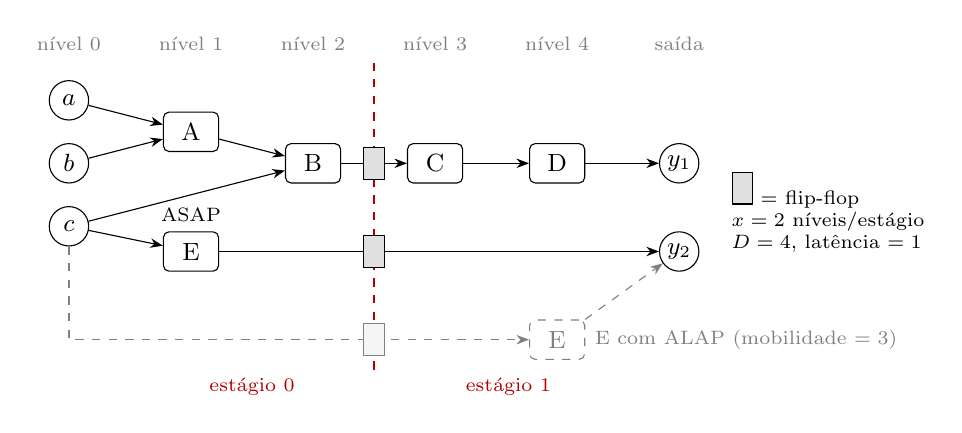
\begin{tikzpicture}[
  lut/.style={draw,rounded corners=2pt,minimum width=7mm,minimum height=5mm,font=\small},
  io/.style={circle,draw,inner sep=1pt,minimum size=5mm,font=\small},
  ff/.style={draw,fill=black!12,minimum width=2.6mm,minimum height=4mm,inner sep=0pt},
  >={Stealth[length=1.6mm]}, x=1.55cm, y=0.8cm]
  % level labels
  \foreach \l in {0,...,4}{\node[font=\scriptsize,gray] at (\l,2.9) {nível \l};}
  \node[font=\scriptsize,gray] at (5,2.9) {saída};
  % nodes
  \node[io]  (a) at (0,2) {$a$};
  \node[io]  (b) at (0,1) {$b$};
  \node[io]  (c) at (0,0) {$c$};
  \node[lut] (A) at (1,1.5) {A};
  \node[lut] (B) at (2,1)   {B};
  \node[lut] (C) at (3,1)   {C};
  \node[lut] (D) at (4,1)   {D};
  \node[lut] (E) at (1,-0.4) {E};
  \node[lut,dashed,gray] (Ealap) at (4,-1.8) {E};
  \node[io]  (y1) at (5,1)  {$y_1$};
  \node[io]  (y2) at (5,-0.4) {$y_2$};
  % edges
  \draw[->] (a)--(A); \draw[->] (b)--(A); \draw[->] (A)--(B); \draw[->] (c)--(B);
  \draw[->] (B)--(C); \draw[->] (C)--(D); \draw[->] (D)--(y1);
  \draw[->] (c)--(E); \draw[->] (E)--(y2);
  \draw[->,dashed,gray] (c.south) |- (Ealap.west); \draw[->,dashed,gray] (Ealap) -- (y2);
  \node[font=\scriptsize,gray,anchor=west] at (Ealap.east) {E com ALAP (mobilidade $=3$)};
  \node[font=\scriptsize,anchor=south] at (E.north) {ASAP};
  % stage cut
  \draw[red!70!black,dashed,thick] (2.5,2.6) -- (2.5,-2.3);
  \node[font=\scriptsize,red!70!black,align=center] at (1.5,-2.55) {estágio 0};
  \node[font=\scriptsize,red!70!black,align=center] at (3.6,-2.55) {estágio 1};
  % registers
  \node[ff] at (2.5,1) {};
  \node[ff] at (2.5,-0.4) {};
  \node[ff,draw=gray,fill=gray!8] at (2.5,-1.8) {};
  \node[font=\scriptsize,anchor=west] at (5.35,0.2) {\begin{tabular}{@{}l@{}}\tikz\node[ff]{}; = flip-flop\\ $x=2$ níveis/estágio\\ $D=4$, latência $=1$\end{tabular}};
\end{tikzpicture}
\end{center}
\vspace{-6pt}

\textbf{Como a ferramenta faz} (\texttt{src/retime.py}).
\begin{enumerate}[label=\arabic*.]
  \item \textbf{Níveis ASAP}: em ordem topológica, as entradas recebem nível 0 e cada LUT recebe
        $1+\max$ dos níveis de seus predecessores. A profundidade $D$ é o maior nível (LUTs no caminho crítico).
  \item \textbf{Níveis ALAP}: em ordem topológica reversa, cada LUT recebe o $\min$ dos níveis de seus sucessores $-1$
        (as saídas ficam em $D+1$). A \emph{mobilidade} $\mathrm{ALAP}-\mathrm{ASAP}$ é a folga da LUT; LUTs críticas têm 0.
  \item \textbf{Estágios}: os níveis são agrupados a cada $x$ níveis (\texttt{--levels-per-stage}) ou em $S$ faixas
        balanceadas (\texttt{--stages}). Cada LUT assume o estágio do seu nível ASAP ou ALAP (\texttt{--policy}).
        As entradas ficam no estágio 0 e as saídas são forçadas para o último estágio.
  \item \textbf{Inserção de registradores}: uma aresta $(u,v)$ recebe $s(v)-s(u)$ flip-flops. Registradores na mesma
        net são compartilhados como uma única cadeia de shift register, então uma net com fan-out paga apenas pelo
        destino mais distante.
  \item \textbf{Exportação e verificação}: a netlist é reescrita em Yosys JSON/Verilog com células \texttt{\$dff} e uma
        porta \texttt{clk}, e comparada à original por simulação ciclo a ciclo com vetores aleatórios.
\end{enumerate}

\textbf{ASAP vs.\ ALAP.} Só as LUTs com mobilidade $>0$ mudam de lugar. O ASAP as puxa para o início, então os
registradores ficam nas suas \emph{saídas} (na figura: E no estágio 0, flip-flop em E$\to y_2$); o ALAP as empurra para
o fim, então os registradores ficam nas suas \emph{entradas} (E tracejada no estágio 1, flip-flop em $c\to$E). O caminho
crítico e a latência são os mesmos; o que muda é o número de flip-flops e o balanceamento de LUTs por estágio, já que o
compartilhamento depende de a net atrasada ter fan-out pequeno ou grande.

\textbf{Escopo.} Trata-se de pipelining baseado em níveis sobre um DAG, com atraso unitário por LUT. O retiming
completo de Leiserson--Saxe (circuitos sequenciais com realimentação, atrasos reais, formulações de período mínimo ou
de número mínimo de registradores) não é abordado.

\end{document}
